
%%%%%%%%%%%%%%%%%%%%%%% file typeinst.tex %%%%%%%%%%%%%%%%%%%%%%%%%
%
% This is the LaTeX source for the instructions to authors using
% the LaTeX document class 'llncs.cls' for contributions to
% the Lecture Notes in Computer Sciences series.
% http://www.springer.com/lncs       Springer Heidelberg 2006/05/04
%
% It may be used as a template for your own input - copy it
% to a new file with a new name and use it as the basis
% for your article.
%
% NB: the document class 'llncs' has its own and detailed documentation, see
% ftp://ftp.springer.de/data/pubftp/pub/tex/latex/llncs/latex2e/llncsdoc.pdf
%
%%%%%%%%%%%%%%%%%%%%%%%%%%%%%%%%%%%%%%%%%%%%%%%%%%%%%%%%%%%%%%%%%%%


\documentclass[runningheads,a4paper]{llncs}

\usepackage{amssymb}
\setcounter{tocdepth}{3}
\usepackage{graphicx}

\usepackage{url}
\urldef{\mailsa}\path|{pmf, md}@tbd.com|
\newcommand{\keywords}[1]{\par\addvspace\baselineskip
\noindent\keywordname\enspace\ignorespaces#1}

\begin{document}

\mainmatter  % start of an individual contribution

% first the title is needed
\title{Foraging in Territories Strange}

% a short form should be given in case it is too long for the running head
\titlerunning{Foraging in Territories Strange}

% the name(s) of the author(s) follow(s) next
%
% NB: Chinese authors should write their first names(s) in front of
% their surnames. This ensures that the names appear correctly in
% the running heads and the author index.
%
\author{P. Michael Furlong%
\and M. D. }
%
\authorrunning{What goes here?}
% (feature abused for this document to repeat the title also on left hand pages)

% the affiliations are given next; don't give your e-mail address
% unless you accept that it will be published
\institute{TBD\\
\mailsa\\
\url{http://www.tbd.com/}}

%
% NB: a more complex sample for affiliations and the mapping to the
% corresponding authors can be found in the file "llncs.dem"
% (search for the string "\mainmatter" where a contribution starts).
% "llncs.dem" accompanies the document class "llncs.cls".
%

\toctitle{Foraging in Territories Strange}
\tocauthor{Furlong \and D.}
\maketitle


\begin{abstract}
The abstract should summarize the contents of the paper and should
contain at least 70 and at most 150 words. It should be written using the
\emph{abstract} environment.
\keywords{foraging, active learning, planetary exploration}
\end{abstract}

%% main text
\section{Introduction}
\label{sec:intro}

Human scientists have become accustomed to such luxuries as breathing, eating
and drinking, and enduring atmospheric and gravitational forces that do not
vary signficantly from ``1''.  Consequently robots have become our scientific
surrogates as we peer into the depths of the ocean or into our solar
neighbourhood.  Travelling to these regions puts stresses on communications
links which in turn limits the situational awarness and reaction times of the
scientists controlling the robot.  For this reason it is important to increase
the ability of robots to make decisions about how to deploy their sampling
capabilities for the purposes of conducting scientific inquiry.

This paper presents an algorithm that enables a robot scientist to use samples
to investigate different classes of objects in order to learn the distribution
underlying that class.  To reflect a science exploration mission the robot has
no global information and cannot return to objects it did not choose to sample.

Why did I do the work?
	Robots exploring the world right now either depend highly on their controllers to give them objectives or they are planning with some global knowledge.  Operating in these kinds of conditions puts constraints on robot exploration opterations by relying on either humans to make decisions or a significant amount of scouting.
	Relying on humans to make decisions means that remote operators require considerable bandwidth to acquire sufficient situational awareness.  Conducting sufficient reconnaissance to make good decisions often obviates the need to send a robotic agent.
	What is lacking in the literature are robots that make decisions about what to investigate \emph{in situ} without reliance on humans and without necessarily having global knowledge.
	
	
What were the central motivations and hypotheses?
	Animals, e.g. human geologists, make decisions about investigating phenomena in the world without necessarily having access to high resolution satellite imagery.  Despite this lack they are able to chose between sampling from materials in front of them and moving on to determine more profitable sampling locations.
	While these decisions may not be globally optimal they do demonstrate an ability that is lacking from exploration robots: to make decisions to stop and engage with the environment or to continue travelling in the hopes of finding more informative sampling locations.




\section{Background}
\label{sec:background}

Automating experiment design is not without precedent.  Kristine Smith started the field of optimal experiment design in 1918.~\cite{smith1918standard}
It is only recently that robots have been employed to conduct scientific exploration autonomously.~\cite{wagner2001science,king2004functional}  Current robot scientists' reliance on global information prevents them from operating in truly unknown environments.  Additionally, previous approaches in sequential decision making from statistics do not necessarily reflect the settings that autonomous robots encounter in the real world.


% Can be compressed/merged with Multi-armed bandit section.
% what is important here is precedent for this type of decision making
% But we don't use any of the results from it.
\subsection{The Secretary Problem}

The secretary problem asks a decision maker to select the best candidate from
sequentially presented candidates where it is not possible to return to
rejected candidates.  In the original setting, there is only one
position for the candidate to fill,~\cite{ferguson1989solved} and the
optimal strategy is to reject the first $\frac{N}{e}$ candidates and then accept
the first candidate who is ranked better than any of the previously seen
candidates.  Further, the decision maker
was able to objectively score the candidates without cost.  In our setting, we do not know the value until sampling, and sampling a class incurs a sampling cost.

% There have been many variations on this problem including selecting multiple
% candidates \cite{vanderbei1980optimal}, or when the total number of candidates
% is random \cite{presman1972best}, for more variations \cite{ferguson1989solved}
% is an excellent source.  What distinguishes the secretary problem from the
% science autonomy problem we propose is that we do not know the value of a
% candidate, or class, when we encounter it.  Additionally repeatedly sampling
% the same class decreases the value to the decision maker. 

\subsection{Multi-armed bandits}

Sequential experiment selection, a type of active learning, is addressed in the
multi-armed bandit (MAB) literature.  This was introduced by Robbins~\cite{robbins1952some} as a means of sequentially selecting which experiments
to conduct with a limited budget.  In Robbins' work,
selecting experiments is modelled on determining the payouts of one-armed
bandit machines -- each machine representing a different experiment.  The player
has a fixed sampling budget and has to sequentially choose which machine to
play, trading off exploiting expected rewards from well-studied arms against
exploring different arms, learning more accurately the payouts of those
arms.  

Lai \emph{et al.}~\cite{lai1985asymptotically} use a value function that sums the mean and the standard deviation of rewards for an arm, in which uncertainty makes an arm more interesting.  Other techniques addressing the exploration/exploitation problem use uncertainty in a reward metric.~\cite{burnetas1997optimal,auer2003using,balcan2006agnostic}  In our setting, because the agent only needs to learn the distribution and not use it for anything, uncertainty is the only necessary reward.

% Lai \emph{et al.} \cite{lai1985asymptotically} introduced the Upper Confidence
% Bound (UCB) rule which values sampling opportunities with the sum of the
% expected reward for a sampling opportunity and a term that tries to balance the
% samples amongst all types of sampling opportunities.
% 
% $$
% Value = \mathbb{E}\left[R_i\right] + \sqrt{\frac{2\ln t_i}{T}}
% $$
% 
% Where $R_i$ is the reward for sampling opportunity $i$, $t_i$ is the number of
% times $i$ has been sampled, and $T$ is the total number of samples distributed.
% Work on proving the bounds of this algorithm has been continued by Agarawal
% \cite{agrawal1995sample} and Auer and Ortner\cite{auer2010ucb}.  
% 
% 
% Other approaches to the bandit problem use reward plus the uncertainty of that
% reward to indicate value.  We see this in the work of Burnetas and Katehakis
% \cite{burnetas1997optimal} and Auer \cite{auer2003using}.  This is a sentiment
% seen in other work, like the optimistic planners of Jurgen Schmidhuber's group
% \cite{schmidhuber1997what,schmidhuber2003exploring,schmidhuber2009simple,sun2011planning}.
% They choose actions that maximize the expected information gain with respect to
% some model they are learning.  The most valuable actions are the ones that
% result in the greatest shift in the distribution the learner is building.
% 
% % This paragraph can go.
% Balcan \cite{balcan2006agnostic} presents a method for learning classifiers by
% requesting samples from the input space with the greatest classification
% error.  Classification error and uncertainty in function value
% are fungible quantities in this case.  An analogy can be drawn between
% the classifiers used in \cite{balcan2006agnostic} and the bandit arms used by
% Auer and Ortner\cite{auer2010ucb}.

% 		- Multi-armed bandit
% 			- Assumes you can access any arm at any time
% 			- Many settings don't have a switching cost between arms.
% 			- Gittins showed that if you have a switching cost and diminishing returns you can solve the problem.
% 			- We say is we will be randomly assigned an arm and a switching cost.

There are a number of distinguishing factors between the MAB setting and the problem explored in this paper.  First, in MAB, the agent
has access to any arm it chooses at any given time.  The arms in MAB are
analogous to the classes in our setting.  The agent in our setting does not get
to choose which of the classes it can investigate.  Any previously seen classes
are no longer available, and new classes arrive per a random model.  Additionally,
the standard MAB setting does not have switching costs, although there are some
formulations which do include such costs.~\cite{jun2004survey}  In our setting, there is a cost incurred
with every choice to continue exploring, and it is a function of the arrival
rates of the different classes.

\subsection{Optimal Foraging}

Foraging is the problem encountered by animals seeking to maximize the intake
of energy when operating in an unknown environment.  The central question to
solving the problem is: Is it more valuable to continue extracting resources
from the current location or to seek out resources in new locations?  Charnov~\cite{charnov1976optimal} introduced a technique for dealing with what he called
``patchy'' environments, in which there are localized regions that contain
different classes of resources.  The forager can
extract value from these patches, with diminishing returns (modeling resources consumed), or choose to
continue to wander randomly through the environment in the hopes of
encountering a more valuable location.

The optimal time to leave the environment, according to Charnov's Marignal Value Theorem, is when the expected return from continuing to
sample from a particular patch is less than the expected return from wandering in the
environment.  In this formulation, the expected return from both the current
patch and the environment are offset by the cost of extracting resources in
this patch as well as the energy spent seeking a new patch.

% 	- Work in the 1970's about foraging.  About making value judgements.  - Key
% 	point from Charnov's work is that there has to be diminishing returns for
% 	extracting from a field (specifically towards an asymptote) - Different from
% 	our setting is that diminishing your reward in one area contributes to
% 	diminishing your reward elsewhere. It isn't like picking apples off one tree,
% 	and finding a new tree with unpicked apples.
% 	\cite{charnov1976optimal}.
 


Pirolli and Card~\cite{pirolli1999information} introduced a model of researchers attempting to
acquire information.  They modelled the rate of information gain and had their
agent decide to leave a patch when the rate of information gain
was lower than that of the environment.  What differentiates their setting from
ours is that their decision maker can choose from which reservoirs to sample.  Our exploring agent does not have that luxury.

% 	- Piroli 1999 - has come up with a very similar formulation as the one that 
% 		Mike and I came up with.
% 		- Something to consider is that we only get to take one sample per patch 
% 			because of science differentiation requirements (i.e. RP can't have 
% 			samples closer than 10cm to each other, maybe as far as 1m)
% 		- We could also incorporate the different cost it takes to identify things 
% 			in the scene.
% 		- We also have different times between patches.
% 		- Should it come to multiple contexts then we have the contextual bandit 
% 			problem
% 				- This means that we could keep different distributions of classes per 
% 					environment.

% Can merge with above.
Kolling \emph{et al.}~\cite{kolling2012neural} studied how humans engage in a gambling task in which players have to consider the option they have before them and the opportunities
the environment provides.  In the described experiment, subjects were repeatedly
presented with a choice of playing a gambling game or being randomly presented
with a different game.  Each game was a Bernoulli trial with some unknown
probability of success.  Kolling \emph{et al.} identify possible neural
substrates for foraging decision making in humans.  The behaviour was near
optimal, with some skewing of probabilities at the extreme ends of the scale,
i.e. $p \approx 0$ or $p \approx 1$.


\subsection{Science Autonomy}

% 	- Yeorger (sp?) WHOI or MBARI has exactly this setup as a problem.
% 	- Thompson, Asher Bender and Stephane Williams Group
% 			- making selections based on maps.  
% 			- Maximum entropy/mutual information smapling.
% 			- They assume global knowledge, we don't have that.  It is reasonable
% 			in many settings of interest, can reduce cost.

Thompson and Wettergreen~\cite{thompson2008intelligent} maximize diversity of
collected samples by using mutual information sampling.  This approach ensures
diversity in the collected sample set, an act that reduces uncertainty in the
input space of a function.  Neither mutual information nor maximum entropy
sampling methods, when used with stationary Gaussian processes, take into
account the dependent variable (the underlying class distribution in our setting) when selecting samples.


Bender \emph{et al.}~\cite{bender2013autonomous} make a modification to that work, instead using Gaussian processes to
identified hypothesized distributions of life across the sea floor to direct
exploratory actions.  The prior maps were generated by vessels passing over the
sea floor prior to the robot's exploration mission, not unlike Thompson and Wettergreen's use of satellite imagery.  The advance of Bender \emph{et al.} is the use of \emph{in situ} measurements to
update the Gaussian process being learned.  Their rover can thus
be said to be generating and testing hypotheses.  However, they are severely
limited by a budgeting size of six ``gulpers'' -- devices for collecting
seawater samples.


Ferri \emph{et al.}~\cite{ferri2010novel} present an approach to prospecting where an autonomous underwater vehicle (AUV) follows a predefined track and needs to decide when to deviate to sample anomalies.  The AUV in this work examines anomalies by engaging in a spiral search pattern, collecting data and characterizing the environment in that location.  In this case, the rover is not limited in its sampling capacity.  However the decision to sample is based on a pre-programmed threshold.  While this may be an excellent way to encode subject matter experts' beliefs on what is interesting, it is fragile in the face of a changing environment and does not adapt to the actual environment the rover encounters.  This exploration problem is an ideal application of the algorithm proposed in this paper.
 
% 
% 	- Previous work in robotic exploration is either dependent on global information or it does not make reasoned decisions about the rest of the world and the sampling opportunities that are immediately available to it.
% 			- opportunistic science only takes advantage of what is immediately availble to the robot and with surplus sampling budget.
% 			- whoi and mbari follow set patterns (which is fine, the lawnmower is a good and noble thing) but they use an arbitrary threshold to make the decision to sample or not.  They do not take into account the rest of the environment.
% 

Likewise, Girdhar \emph{et al.}~\cite{girdhar2013autonomous} present an approach to autonomous exploration wherein a robot
investigates a scene when it encounters phenomena that do not reflect its
current model of the world.  Specifically, they use topic models to describe
scenes and sample when they encounter scenes that do not fit into the topic models
they have constructed.  In these works, the vehicle has no limit on its sampling
capacity and is always collecting data.  By slowing the vehicle down, more
samples are collected in anomalous scenes.  In this fashion this is very
similar to later work by Thompson \emph{et al.}.~\cite{thompson2013adaptive}

Additionally, Girdhar \emph{et al.} build upon their anomaly detection techniques to develop a path planning method to maximize
information gain of paths.~\cite{girdhar2014curiosity}  In that respect, it
belongs with the family of curiosity-driven algorithms pioneered by
Schmidh{\"u}ber \emph{et al.}. 
% \cite{schmidhuber1997what},
% \cite{schmidhuber2003exploring}, \cite{schmidhuber2009simple},
~\cite{sun2011planning}  The fundamental concept behind these approaches is
that an explorer should spend its time investigating regions of the world (or
hypothesis space) where its models are the least certain.

% \subsubsection{Our Prior Work}

Previous work by the primary author with optimal foraging for science autonomy has considered robots with limited sampling budgets~\cite{furlong2014budgeting} and assumed knowledge of the number of sampling opportunities that would occur.  While the limited sampling budget is realistic, the foreknowledge of the transect is not necessarily so.  This paper improves upon the prior work by using productivity to reason about sampling choices and gives a constraint of time instead of an unknowable number of sampling opportunities.

% 		- Apply optimal foraging, specifically Charnov's marginal value theorem
% 		model of foraging to the problem of science autonomy* in the following setting:	
% 			- Limited sampling budget
% 			- Attempting to learn distributions not acquire quantities of some object.
% 			- Trying to learn information objectively without an objective. 
% 			- Can't know the reward until you sample.
% 			- It's a fusion of bandits and foraging.  The fact that we are focusing on gaining information gives us diminishing returns which lets us use 
% 			- Don't have access to all the arms at any given time, which is what makes it a foraging problem.
% 			- Don't have the choice of what objects you encounter.

As explained, real robots may not be able to predict the rewards they will earn from their actions and have to deal with unreliable arrival rates for sampling opportunities.  These are concerns that are not modelled in typical sequential experiment selection algorithms such as the multi-armed bandit or secretary problems.  This motivates the problem setting used in this paper, described in detail in the following section.


\section{Method}
\label{sec:method}

The decision making agents in this paper are tested on several randomly
generated transects.  They are repeatedly presented with an object to sample
and have to make the choice to either take a sample or continue travelling
along the transect.  Like the Robbins' secretary problem the agents are not
permitted to backtrack to avail of a previous opportunity.


Figure \ref{fig:transect} gives an example of a simulated transect. As we can
see there are sampling opportunities of different types scattered along the
path that the robot travels along.  

\begin{figure}[htpd!]
	\centering 
	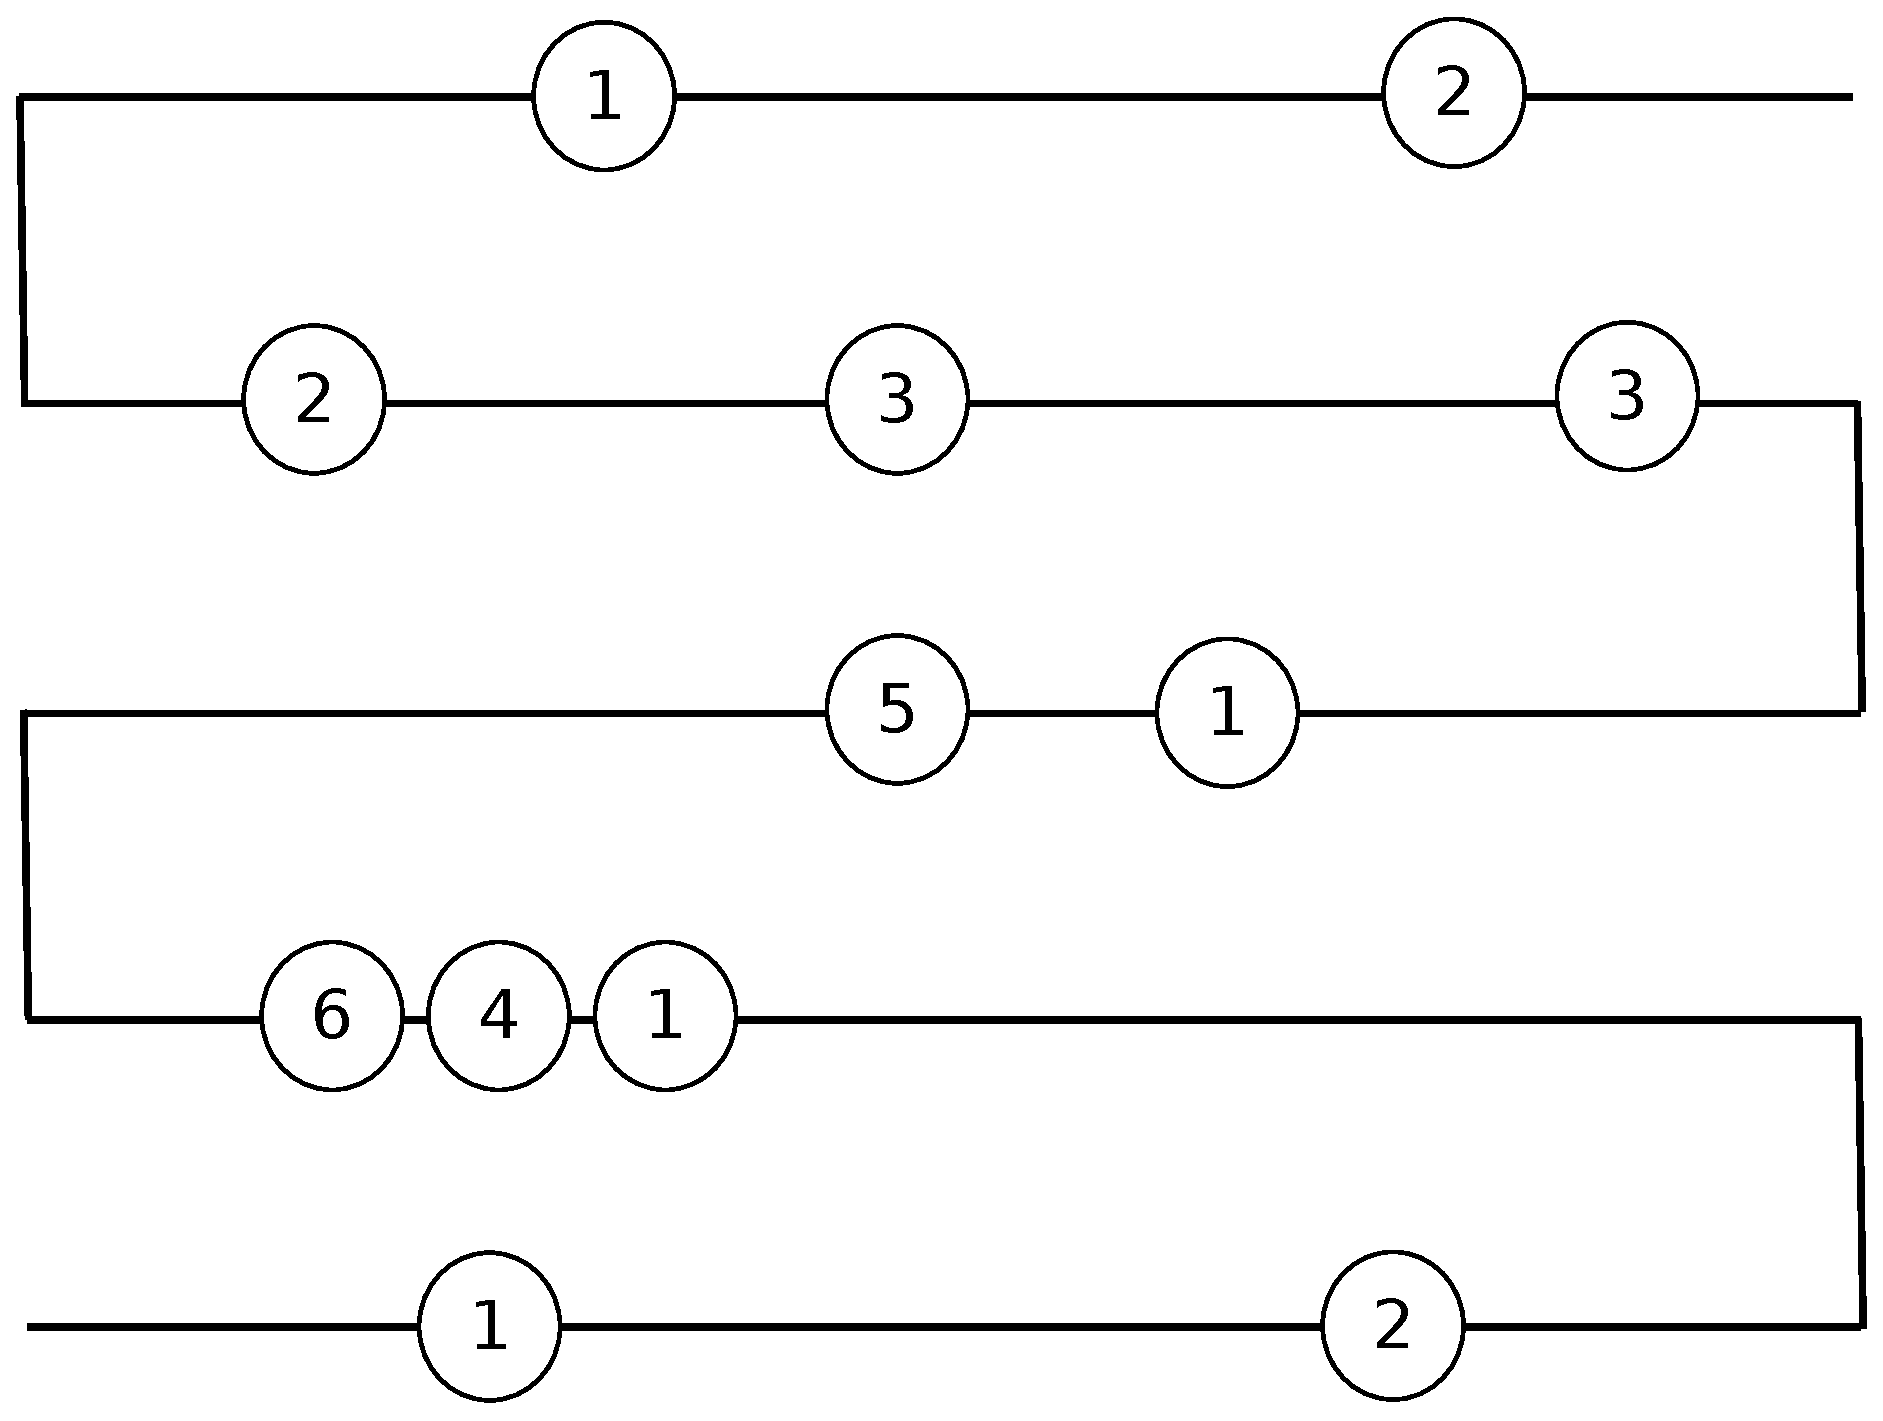
\includegraphics[width=0.8\textwidth]{transect}
	\caption{A cartoon illustrating a transect a robot might be encountering and how samping opportunities of different types may be distributed along it.  In the field the robot would start at one end of the path and follow it to the other end.  There is one path that the rover may follow across the terrain resulting in it encountering different types of sampling opportunities.}
	\label{fig:transect}
\end{figure}


The primary objective of the robot is to learn distributions behind different
classes of objects.  For example they may be the probability distribution
governing the density of sub surface microbial life in different classes of
soil.  Previous work have identified that texture information can successfully
classify different types of soil material \cite{dunlop2006automatic}.  
We imagine that the classes of objects in
this research could correspond to those soil classes.


\subsection{Experiment}

The experiment presented in this paper is a modification of the experiments
presented in \cite{furlong2014sequential} and \cite{furlong2014budgeting}.  In
the prior work agents were equipped with limited sampling budgets.  In this
experiment the agents have an unlimited capacity to take samples, but the time
to take the sample is non-zero and there is an overall limit on the duration of
the mission.  The sampling cost and the overall mission time is given in units of arbitrary time.

As with the previous experiments the agents are not permitted to back track in
the hopes of getting a better opportunity.  The primary reason is to constantly
drive the robot to the end of its exploration mission.  Coverage is an
important part of exploration and permitting.  Additionally making decisions
between a current opportunity, a hypothetical future, and any number of
previously seen but unsampled opportunities is considered a more complex
problem and outside the scope of this paper.

In the experiment there are six different classes of objects the agent may
encounter.  They each have their own arrival rate and their appearance along
the transect are generated with a poisson process.  In this paper the arrival
rates of the different sampling opportunities do not change over the course of
the experiment.  While this is almost certainly not the case for long range
traversals like those seen in the Life in the Atacama Desert Project it is a
reasonable approximation for shorter-range traverses.

\begin{table}[htpd!]
	\centering
	\begin{tabular}{l|ccc}
		Class & Mean & Standard Deviation & Arrival Rate\\
							 & (arbitrary units )  & (arbitrary units) & (arbitrary time)\\
 		\hline
		1 & 0 & 1 & 1\\
		2 & 10 & 0.1 & 0.8 \\
		3 & 0 & 5 & 0.9\\
		4 & 2 & 4 & 1.1\\
		5 & -2 & 4 & 0.05\\
		6 & 0 & 0.1 & 1.1\\
		\hline 
		\\
	\end{tabular}
	\caption{The classes the robot is investigating all have values derived from Gaussian random variables with means and standard deviation given.  Different instances of those classes are encountered in accordance to a Poisson process with the rates specified in the above table.  The units of the distribution's mean and variance can be ignored for the purposes of this experiment.  The arrival rate in this experiment is given in units of arbitrary time.  All time quantities -- arrival rate, mission time, and sampling cost -- can be scaled to the order of the mission at hand.}
	\label{tbl:classes}
\end{table}

\subsection{Algorithms}

	% This is only relevant in the larger work.
	% - figure method.3: texture cam, raw image and texture labelled image.

	The experiment builds on prior work.  Here we present two algorithms that are being testing on the simulated transect described above.

\subsubsection{Uniform Sampling}

The Uniform Sampling algorithm attempts to distribute the number of samples it
can collect evenly between the different types of objects present on the
transect.  This is chosen because it was a robustly successful algorithm, as
seen in the prior work \cite{furlong2014sequential} and \cite{furlong2014budgeting}.

The Uniform Sampling algorithm does not consider the time remaining in the
transect, nor the time to complete sampling.  In this setting the algorithm
chooses to sample a class either if it does not have the most samples of all
the encountered classes or if is the max and all other classes have been
sampled an equal number of times.

\subsubsection{Foraging}

The foraging algorithm is an attempt to maximize the productivity of the learning agent along the transect.  We attempt to maximize the number of bits learned per unit time.

The reward for sampling a class is an analog for the definition of surprise as
defined by the Koch et al {cite papers}.  Koch looked at the change in the
distribution that resulted in a Bayesian update.  Because this work uses a
non-parametric kernel density estimation we compare
$\log\left(\frac{\hat{p}(x|D\cup \left\{x\right\})}{\hat{p}(x|D)}\right)$.  To
be compatiable with optimal foraging algorithms, specifically the Marginal
Value Theorem of Charnov \cite{charnov1973optimal} the reward function must
have dimishing returns.  In the case of information update the Bayes Factor
will eventually converge to approximately 1, likewise our estimated empirical
bayes factor.  We take the log of this approximation such that it converges to
zero as more samples are collected.


	- figure method.2: The reward function as samples are given to it, for two or three different distributions.

\begin{figure}[htpd!]
	\centering
	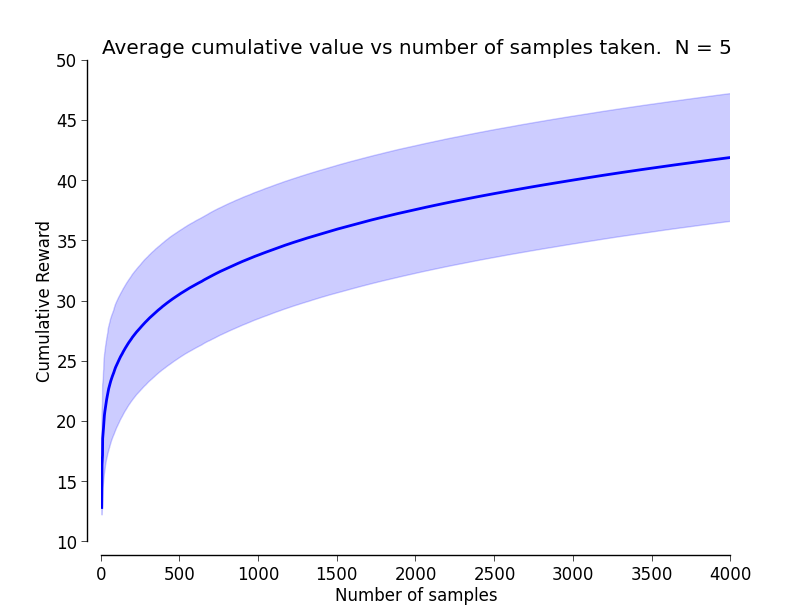
\includegraphics[width=0.8\textwidth]{images/cumulative-reward.png}
	\caption{The reward function plotted is the cumulative reward for sampling from a Gaussian distribution with mean 0 and variance 1.  The cumulative reward is averaged over five trials of 4000 samples.  As the number of samples from a distribution is increased the amount of information gained is reduced.  The reward at any point in time can be viewed as the reduction in Shannon surprise of an instantiation of the random variable as a result of incorporating that value into the learned distribution.  It is important to note that the returns of this reward function decrease with the time spent sampling a particular random variable.  The diminishing returns are necessary to use the Marginal Value Theorem formulation from Charnov \cite{charnov1973optimal}.}
	\label{fig:reward}
\end{figure}

	- Combining foraging models with bandit literature 
		- The previous work on foraging assumed an inherent value to
			options that the agent cared about.  Specifically, energy stored up.
		- We use a valuation model taken from bandit literature.  
		- We use the reward function from Koch's attention models
		- We use the decision making process from foraging. 
		- We add the concept of multi-arrival rate things, awareness of time limits.
	- Previous work had a limit on the number of samples it could take
		- We realized that the actual quantity that limits the exploration process
			is time.
		- By limiting the time and (in this case) relaxing the limit on sample sizes we more accurately deal with productivity.  
	- This experiment models a type of prospecting where the number of samples isn't limited but they do take time. 
	- To that end we are looking at productivity.

	-  This experiment is more akin to contextual bandits.  
	- The image represents a context, the NIRVSS 
	- Apply texturecam classification of a scene, as the context
	- the choice is to sample or continue

	- Productivity 



\section{Results}
\label{sec:results}


- Figure results.1: Overall error at the end of the trial with unlimited sampling and without weighing by the rarity (1/prob of occurrence) of the class
- Figure results.2: overall error at the end of the trial with unlimited sampling and with weighing by the rarity of the class
- Figure results.3: Overall performance when combining limited time and limited sample budgets.

% Different arrival rates and different distributions.

\begin{figure}[htpd]
	\centering
	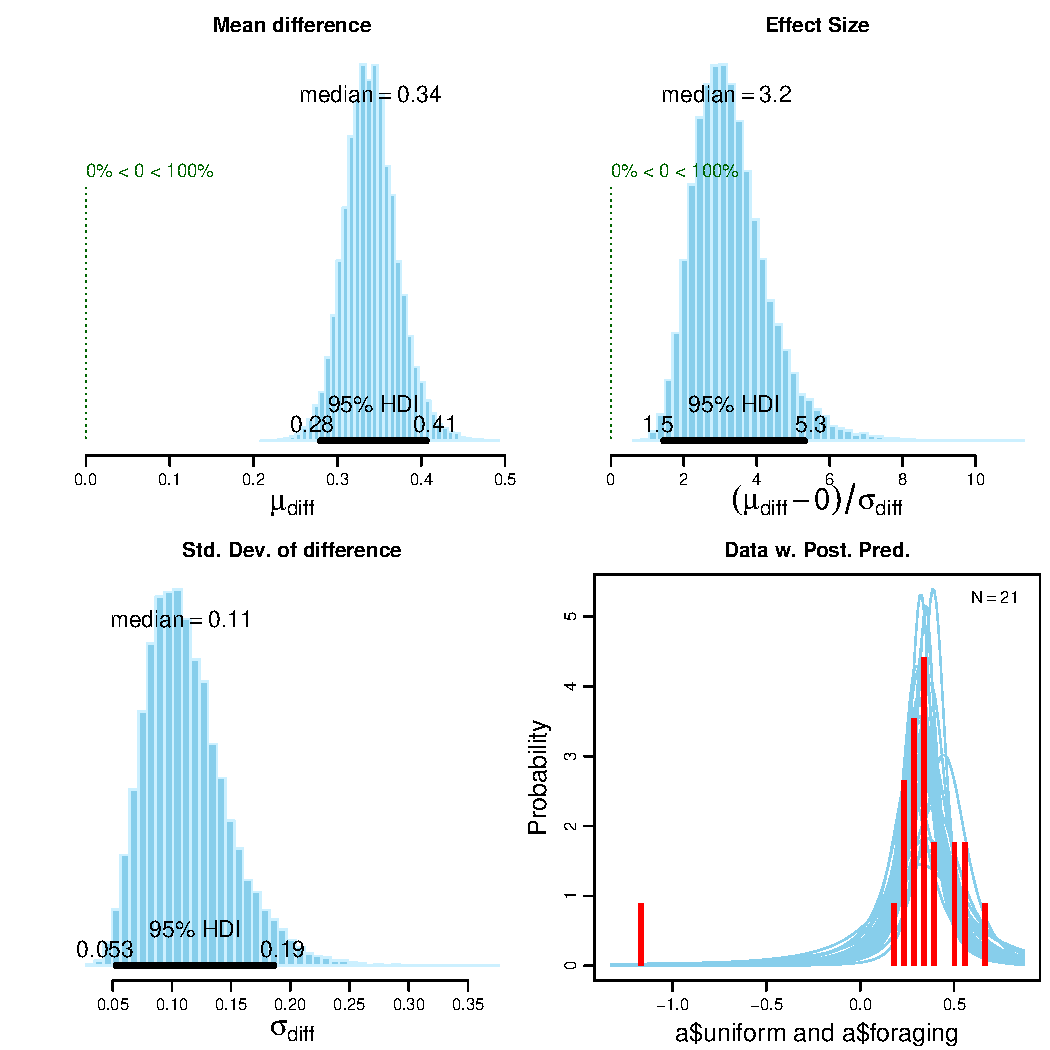
\includegraphics[width=0.8\textwidth]{images/diff-diff.pdf}
	\caption{Analysis of the basic scenario with different arrival rates and standard deviations.}
	\label{fig:diff-diff}
\end{figure}

\section{Conclusion}
\label{sec:conclusion}

In this paper we present a new algorithm created by combining sequential experiment selection and models of optimal foraging with an information theoretic reward function.  For certain regimes of operation the new algorithm is significantly better the control algorithm based on optimal experiment design alone.  Additionally this work continues the process of introducing sequential selection to the field of science autonomy.  

From the experiment presented in this paper we can conclude three things.  First, for small sampling costs relative to the transect duration the foraging algorithm produces about a 50\% reduction in accumulated error.  For the small sampling costs the effect size is substantial and our Bayesian paired t-test gives us 95\% confidence that the increase in performance is non-zero.

Second, when the sampling cost is large relative to the duration of the transect Uniform sampling is as good as or better than foraging.  This makes sense, as the first samples one collects are the most informative about a distribution.  Distributing samples across the different classes of objects increases the overall rate of information gained, ensuring the greatest short-term reduction in error.

Thirdly, when the sampling cost gets sufficiently large foraging again becomes a competative algorithm.  The convergence in performance is mainly due to the very limited ability to sample and consequent poor performance of both algorithm.  

This work does not address perception and requires some system to parse scenes to identify the classes available to the robot.  This is necessary for fielding this algorithm on a robot.  The algorithm does not account for the following deviations in the problem setting: If there is more than one type of sensor with a different cost to use; Class arrival rates that change over time; Class distributions changing over time.  These need to be addressed in the future to make a more plausible robot scientist.  It is the desire of the authors to make the agent responsible not just for collecting data, but to generate and test hypotheses about the environment.
% 
% 1. Implement on a real robot (of course).  Integrate some sensor processing algorithm (texturecam?) to abstract from images/whatever to categories as used in this paper.
% 
% 2. Multi-objective optimization (different sensors with different costs)
% 
% 3. Vary the arrival rates much more (have sims set up for that, haven't finished executing them yet.  Seriously! Yes, yes, write it in C next time.)
% 
% 4. Handle when the distributions change. 
% 
% 5. Handle when arrival rates change.






\bibliography{merged}

\appendix

\end{document}
